\section{Pure Shift NMR}

\subsection{The \acl{2DJ} Experiment}
The \ac{2DJ} experiment\cite{Aue1976, Morris2009} provided the first means of
achieving pure shift spectra. It has a simple pulse sequence, presented in
Figure \ref{fig:pure_shift_seqs}.a; after excitation of magnetisation onto the
transverse plane, the indirect dimension evolution consists of a spin echo, with
acquisition following immediately afterwards. Fourier transformation in both
dimensions leads to a spectrum in which only scalar couplings contribute in
$\Fone$, as the chemical shifts are refocussed by the spin echo, while both
scalar couplings and chemical shifts contribute in $\Ftwo$.
Peaks belonging to a particular multiplet lie along a line at \ang{45} to the
$F^{(1)}$ and $F^{(2)}$ axes, as seen in panel a. of Figure
\ref{fig:jres_spectrum}.
\begin{figure}%
    \centering%
    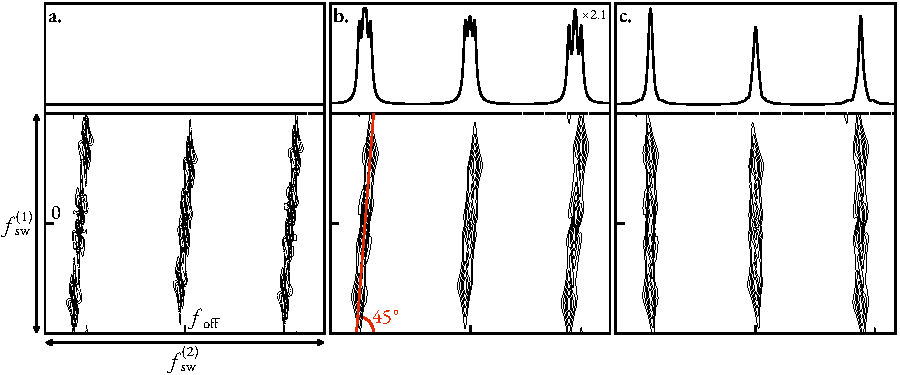
\includegraphics{jres_spectrum/jres_spectrum.pdf}%
    \caption[
        Example of a simple \acs{2DJ} spectra derived from an AMX spin system,
        processes in different ways.
    ]
    {%
        Example of a simple \acs{2DJ} spectrum derived from an AMX spin system.
        Each panel showcases the appearance of the spectrum following different
        processing procedures. Below: contour plots of the spectrum. Above: the
        summation of the spectrum along the indirect axis.
        \note{Put 45 line on panel a}
        \textbf{a.} Spectrum produced from sine-bell apodisation followed by
        \ac{FT} in both dimensions, which features phase-twist peaks, and which
        sums to zero along the indirect dimension. Each multiplet lies along a
        line at \ang{45} to the $F^{(1)}$ and $F^{(2)}$ axes. Note that this
        line often appears to make an angle that is greater than \ang{45} with
        the $F^{(2)}$ axis when viewing spectra, due to the relative scaling of
        the frequency axes (typically, $\fswtwo \gg \fswone)$.
        \textbf{b.} Magnitude-mode spectrum produced from \textbf{a.} by
        subjecting each point to $\sqrt{\Re(x)^2 + \Im(x)^2}$.
        \textbf{c.} Spectrum generated after application of a \ang{45} shear to
        \textbf{b}.  The summation produces a pure shift spectrum, though this
        features peaks with broad wings, and significant non-linearities.
   }%
    \label{fig:jres_spectrum}%
\end{figure}%

An FID generated by the \ac{2DJ} experiment is hypercomplex, taking the form of
\eqref{eq:general-fid} with $D=2$ and $\zeta^{(1)} = \exp(\iu\cdot)$, i.e.
\begin{equation}%
    \begin{split}%
        \jresfid\idxnonentwo =
        \sum_{m=0}^{M-1} \bdam \exp\left( \iu \bdphim \right)
            \exp\left(\left(2 \pi \iu \bdfonem
            - \bdetaonem\right) {\none}_{\vphantom{t}} \Dtone\right) \times \\
            \exp\left(\left(2 \pi \iu  \left(
            \bdftwom - \fofftwo \right)
            - \bdetatwom\right) {\ntwo}_{\vphantom{t}} \Dttwo\right)
            + \symbf{W}\left[n^{(1)}, n^{(2)}\right].
    \end{split}%
    \label{eq:jres-fid}
\end{equation}%
The transmitter offset term has been neglected in the indirect dimension, since
chemical shift evolution does not occur.
For each signal in the \ac{FID}, the indirect- and direct-dimension
frequencies are intimately linked by the relations
\begin{subequations}
    \begin{gather}
        \bdfonem = d_m,\\
        \bdftwom = c_m + d_m,
    \end{gather}
    \label{eq:f1-f2-2dj}
\end{subequations}
where $c_m$ is the Larmor frequency of the spin giving rise to the $m$\textsuperscript{th} signal, and $d_m$ is the displacement of the signal from $c_m$, as a result of scalar couplings\footnote{
    $d_m$ will be a linear combination of all the scalar couplings associated
    with the spin giving rise to the signal, with all the coefficients being
    $\pm \nicefrac{1}{2}$.
}.
$c_m$ can be thought of as the ``central frequency'' of a particular multiplet structure in the dataset.

The major downside of the \ac{2DJ}
experiment is there is no means of generating a pair of phase- or
amplitude-modulated signals which are the conventional route to
frequency-discriminated spectra with absorption mode lineshapes, as no mixing
time exists in the pulse sequence. The FT of $\jresfid$ produces a spectrum
$\jresspec$ with phase-twist peaks,
which possess contributions from both absorption and dispersion Lorentzians (Figure \ref{fig:jres_spectrum}.a).
As with other experiments which produce hypercomplex signals, such as
\ac{COSY}, the data is conventionally displayed in ``magnitude-mode'', in which
the absolute value of each point in the spectrum is plotted.

There are two primary steps involved in obtaining a
pure shift spectrum from $\jresspec$:
\begin{enumerate}
    \item Perform a \ang{45} shear (often called a tilt) on the spectrum array,
        leading to the separation of chemical shifts and scalar couplings onto
        orthogonal axes  (Figure \ref{fig:jres_spectrum}.b). Each
        slice in $\Ftwo$ is subjected to a right circular rotation such that
        \begin{subequations}
            \begin{gather}
                \jresspectilt\left[{\none}\vpsub{\mathrm{sw}},{\ntwo}\vpsub{\mathrm{sw}}\right] =
                \jresspec\left[{\none}\vpsub{\mathrm{sw}},\ntwonew\right],\\
                \ntwonew = \left(
                    {\ntwo}\vpsub{\mathrm{new}} + \left\lfloor
                        \frac
                            {\fswone \Ntwo\vpsub{\mathrm{sw}}}
                            {\fswtwo \None\vpsub{\mathrm{sw}}}
                        \left(
                            \frac{\None\vpsub{\mathrm{sw}}}{2} - \none
                        \right)
                    \right\rceil
                \right) \bmod \Ntwo.
            \end{gather}
        \end{subequations}
        This achieves the mapping $\jresspec\left(\fone,\ftwo\right)
        \rightarrow \jresspec\left(\fone, \ftwo - \fone\right)$ which, as can
        be seen from \eqref{eq:f1-f2-2dj}, leads to a spectrum in which all
        peaks belonging to a particular spin being located at the same
        frequency in $\Ftwo$.  The effectiveness of the shear is maximised when
        both $\nicefrac{\fswtwo}{\fswone}$ and $\nicefrac{\Ntwo}{\None}$ are
        powers of 2\note{check this}.
    \item Sum the spectrum along $\Fone$:
        \begin{equation}
            \specps\idxntwo =
            \sum_{\none=0}^{\None-1} \jresspectilt\idxnonentwo.
        \end{equation}
\end{enumerate}%
If the spectrum wasn't in magnitude-mode, shearing and summing would lead to
the absorptive and dispersive components of the spectrum cancelling each other
out, such that the zero vector would be obtained.
With a magnitude-mode spectrum, the process leads to undesirable pure shift
spectra with broad ``wings'', and non-linearities\note{Ask about what this
means exactly} on account of the presence of dispersive
character. The dispersive component can be suppressed by appropriate processing
to make the FID envelope symmetric in both dimensions, such as with sine-bell
apodisation or pseudo-echo reshaping\cite{Bax1981}, though this results in a
significant reduction in sensitivity being incurred.
\begin{figure}
    \centering
    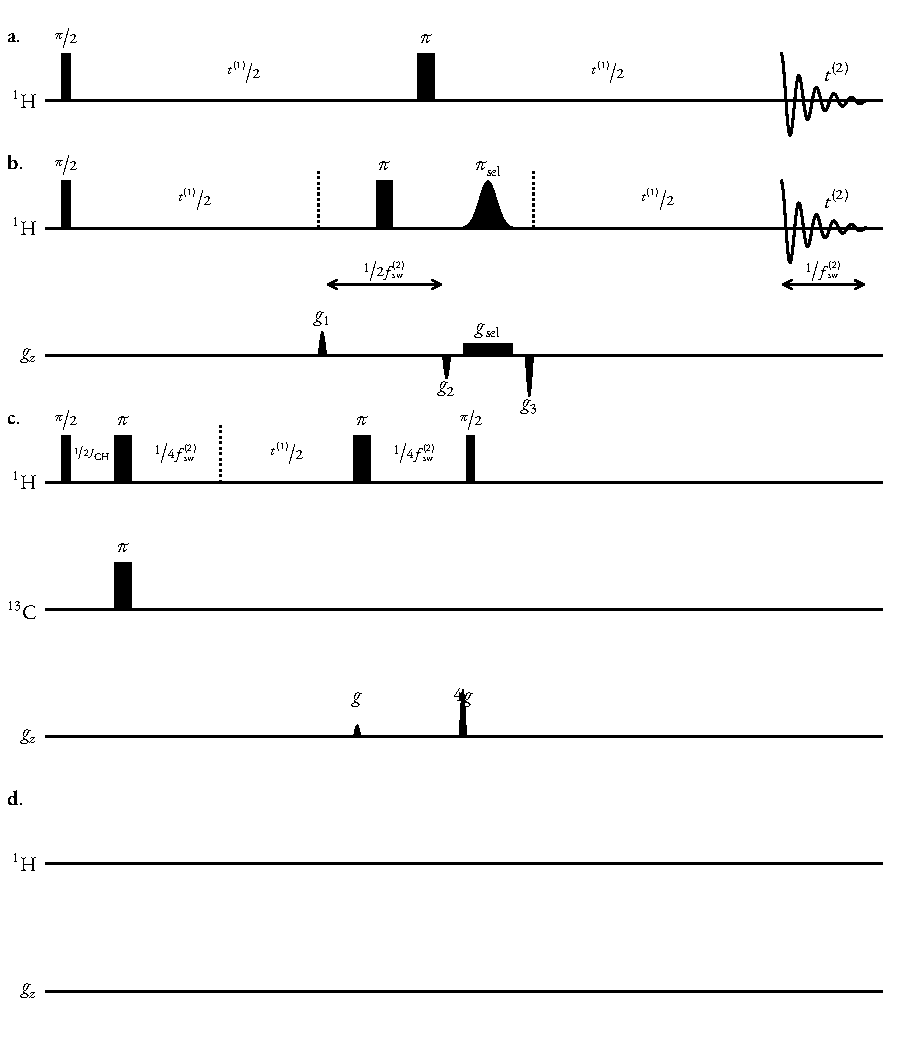
\includegraphics{pure_shift_sequences/pure_shift_sequences.pdf}
    \caption[
        The pulse sequences of some common pure shift experiments.
    ]{
        \note{Work needed. Figure out the correct delays in ZS, BIRD, PSYCHE}
        The pulse sequences of four of the most common pure shift experiments.
        \textbf{a.} \acs{2DJ}.
        \textbf{b.} The \acs{ZS} method.
        \textbf{c.} The \acs{BIRD} method.
        \textbf{d.} The \acs{PSYCHE} method.
    }
    \label{fig:pure_shift_seqs}
\end{figure}

\subsection{The \acl{ZS} Method}
\label{subsec:ZS}
Zangger and Sterk introduced a pulse sequence element which achieves
\emph{slice-selective excitation}, by applying a low \ac{RF} power (weak) \ang{180}
pulse\footnote{Conventionally, a R-SNOB pulse is used\cite{Kupce1995}.} in the
presence of a \ac{PFG} along the $z$-axis\cite{Zangger1997}. Such an element
excites a
given spin only in a narrow range of heights in the sample, as the \ac{PFG}
induces a shift in resonance frequency according to $\Updelta \omega(z) = \gamma
gz$, where $g$ is the magnitude of the \ac{PFG}. By placing a hard
\ang{180} pulse adjacent to the selective pulse, the
``active'' spin in a given slice is rotated by \ang{360} (i.e. no net
rotation), while all other (``passive'') spins are only rotated by \ang{180}.
Placing such a element in the middle of the $\tone$ evolution therefore
achieves refocussing of the J-couplings associated with the active
spin\cite{Aguilar2010}. In order to achieve effective decoupling of any given
pair of spins, it is necessary that the bandwidth of the selective π-pulse is
smaller than the difference in their Larmor frequencies. However, with more
selective pulses, a smaller proportion of the available spin magnetisation will
contribute to the final FID, and hence sensitivity will be diminished
\footnote{
    The reduction in sensitivity is $\propto \nicefrac{f_B}{\gamma G_z l_z}$,
    where $f_B$ is the selective pulse bandwidth, and $l_z$ is the length of
    the sample lying within the receiver coil ($\approx
    \qty{1.5}{\centi\meter}$).
}.
Therefore a trade-off exists between effective decoupling of all spins, and
achieving the greatest sensitivity possible. In the case of strong coupling,
the \ac{ZS} method tends to perform poorly relative to other options for this
reason. The \ac{ZS} element has utilised in order to generate \ac{2DJ} datasets
comprising phase-modulated pairs, enabling the generation of pure
absorption-mode spectra\cite{Pell2007}. Pure shift spectra with far more
desirable lineshapes can be achieved relative to using a typical magnitude-mode
spectrum \ac{2DJ}, though with a significant loss of sensitivity.

\subsection{The \acs{BIRD} Method}
The \ac{BIRD} pulse sequence element\cite{Garbow1982,Bax1983} also takes
advantage of the idea of selectively inverting passive spins, while leaving
active spins unaffected.
However the active spins are those which are directly bound to a low natural
abundance
heteronucleus, with the two most common heteronuclei used being \textsuperscript{13}C (1.1\% abundance) and \textsuperscript{15}N (0.37\% abundance)
The passive spins are those bound to far more abundant nucleus (i.e.
\textsuperscript{12}C or \textsuperscript{14}N). The reduction in sensitivity
of the experiment relative to a full-sensitivity experiment is therefore known
and constant across samples. In scenarios where strong coupling exists, \ac{BIRD} can
achieve improved sensitivity over \ac{ZS}, since with the latter a very weak
selective pulse would be required to ensure it is of a sufficiently small
bandwidth. The \ac{BIRD} method is particularly attractive in scenarios where
the sensitivity penalty due to the involvement of a low-abundance nucleus has
already been paid, for example in sequences where an \ac{INEPT} block is present.\note{CITATIONS}

\subsection{\acs{PSYCHE}}
\label{subsec:psyche}
\note{TODO}
\ac{PSYCHE}
Original paper\cite{Foroozandeh2014}, tutorial paper\cite{Foroozandeh2018},
PSYCHE-2DJ\cite{Foroozandeh2015,Kiraly2017}: note that this is a 3D experiment therefore long
run time.

\subsection{Pure shift spectra from 2DJ estimation}

Procedures based on the estimation of \ac{2DJ} datasets have been
presented previously. Nuzillard introduced
\ac{ALPESTRE}\cite{Nuzillard1996,Martinez2012}, in which
the parameters of each indirect-dimension FID are estimated using \ac{LPSVD},
such that a set of parameters $\symbf{\Theta} \in \mathbb{R}^{\Ntwo
\times 4M}$ is generated.
\begin{equation}
    \symbf{\Theta}\left[\ntwo\right] =
    \begin{bmatrix}
        \left[\bda^{\vphantom{(1)}}_{\ntwo}\right]\T &
        \left[\bdphi^{\vphantom{(1)}}_{\ntwo}\right]\T &
        \left[\bdfone_{\ntwo}\right]\T &
        \left[\bdetaone_{\ntwo}\right]\T
    \end{bmatrix}\T.
\end{equation}
The parameters generated are used to propagate each FID backward into
$-\tone$, producing a ``full-echo'':
\begin{equation}
    \begin{split}
        \symbf{Y}_{\text{full}}\left[\none, \ntwo\right] = \sum_{m=0}^{M-1}
            \bda_{\ntwo} \left[ m \right]
            \exp\left(\iu \bdphi_{\ntwo} \left[ m \right] \right)
            \exp\left(\left(2 \pi \iu \bdfone_{\ntwo} \left[ m \right] \none
            -\bdetaone_{\ntwo} \left[ m \right] \left\lvert \none \right\rvert \right)\Dtone\right), \\
        \forall \none \in \lbrace -\None + 1, \cdots, 0, \cdots, \None - 1 \rbrace,\ \forall \ntwo \lbrace 0, \cdots, \Ntwo - 1 \rbrace.
    \end{split}
    \label{eq:full-echo}
\end{equation}
\ac{FT} of \eqref{eq:full-echo} generates a spectrum whose real component comprises absorption-mode
Lorentzian character in both dimensions. This opens up the means of producing
pure-shift spectra from the \ac{2DJ} experiment with sharp lineshapes and
without signal loss. A similar approach proposed by Mutzenhardt et al.
instead constructed full echoes via \ac{LP} of each direct-dimension
\ac{FID}, and generation of a full echo by propagating
into $-\ttwo$\cite{Mutzenhardt1999}.


